
\documentclass[12pt,epsfig,color,russian]{article}
\usepackage[russian]{babel}
\usepackage{epsfig}
\usepackage{color}

\topmargin=0cm
\hoffset -30mm
\voffset -12mm
\setlength{\unitlength}{1mm}
\parindent=10mm
\textheight=250mm
\textwidth=190mm
\pagestyle{empty}

\begin{document}
\sf\Large


\centerline{\underline{\Huge\bf РАБОТА и ЭНЕРГИЯ}}
\hspace{3mm}
Сила $\vec{f}$ вызывает перемещение тела. Характеристика ее действия -- это РАБОТА {\sl (\underline{A}ction)}.\\
 \setlength{\unitlength}{1mm}
  \begin{picture}(190,50)(0,0)
   %\put(0,0){\framebox(190,40)[b]{}}
   \put(0,5){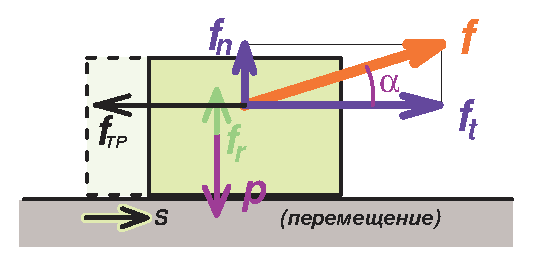
\includegraphics{GP004F01.eps}}
   \put(190,0){\makebox(0,0)[br]{\parbox{100mm}{
   Не вся сила {\color{red}$\vec{f}$} принимает участие в перемещении тела, а только ее составляющая в направлении перемещения ${\color{blue}\vec{f_t}}$:\hspace{5mm} $f_t=f\cdot\cos\alpha$
   \begin{displaymath}
   A=S\cdot f_t = S\cdot f\cdot\cos\alpha = \left(\vec{f}\cdot\vec{S}\right)
   \end{displaymath}
   }}}
  \end{picture}\\
 Здесь вертикальная составляющая $\vec{f_n}$, вес тела $\vec{p}$ и реакция опоры $\vec{f_r}$ никакой работы не производят. Сила трения $\vec{f_{TP}}$ делает {\bf отрицательную} работу, по\-скольку направлена противоположно движению: $\left(\vec{f_{TP}}\cdot\vec{S}\right)<0$.\\[1mm]

 Если сила не постоянна, а меняется во время движения:\\
 \setlength{\unitlength}{1mm}
  \begin{picture}(190,70)(0,0)
   %\put(0,0){\framebox(190,70)[b]{}}
   \put(0,0){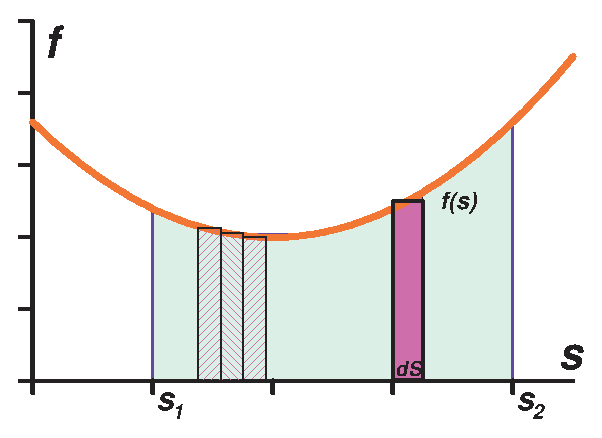
\includegraphics{GP004F02.eps}}
   \put(190,0){\makebox(0,0)[br]{\parbox{80mm}{
   Разобьем весь путь ($S_2-S_1$) на малые отрезки $dS$ и на каждом из отрезков посчитаем работу:
   \begin{displaymath}
   dA= \left(\vec{f}\cdot\vec{dS}\right)
   \end{displaymath}
   а затем все это просуммируем:
   \begin{displaymath}
   A=\int_{s_1}^{s_2} \left(\vec{f}\cdot\vec{dS}\right)\simeq\sum_i\left(f_i\cdot dS_i\right)
   \end{displaymath}
   }}}
  \end{picture}\\[1mm]
  \begin{picture}(190,64)(0,0)
   %\put(0,0){\framebox(190,60)[b]{}}
   \put(0,0){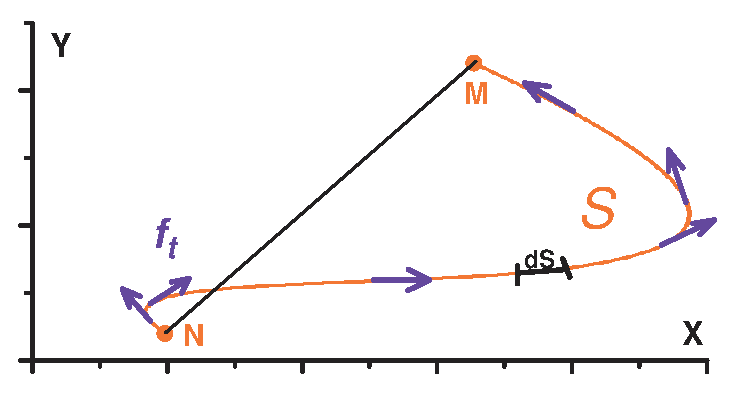
\includegraphics{GP004F03.eps}}
   \put(190,-2){\makebox(0,0)[br]{\parbox{60mm}{Для криволиней\-но\-го движения надо ин\-те\-гри\-ровать (сум\-ми\-ро\-вать) по пути $S$, а не по смещению $NM$:
   \begin{displaymath}
   A=\oint_{N}^{M} \left(\vec{f}\cdot\vec{dS}\right)=
   \end{displaymath}
   \begin{displaymath}
   \oint_{N}^{M} \left(f_xdx+f_ydy+f_zdz\right)
   \end{displaymath}
   }}}
  \end{picture}

\underline{\bf Мощность}
\begin{center}
\fbox{\parbox{180mm}{\color{blue}\bf Физ. величина, пропорциональная работе и обратно пропорциональная тому времени, за которое она совершена.}}\\[1mm]
\end{center}
Средняя мощность за промежуток времени $\Delta t$:
   \begin{displaymath}
   W=\frac{\Delta A}{\Delta t}=\frac{f\cdot \Delta S}{\Delta t}
   \end{displaymath}
Мгновенная мощность в данный момет:
   \begin{displaymath}
   W(t=\tau)=\lim_{\Delta t\rightarrow 0}\frac{\Delta A}{\Delta t}=\frac{dA}{dt}=f_t\cdot\frac{dS}{dt}=\left(\vec{f}\cdot\vec{v}\right)
   \end{displaymath}

\underline{\bf Единицы работы и мощности}
\begin{itemize}
\item CGS: $[s]$ = см, $\;\;\;\;[f]$ = дина = г$\cdot$см/с$^2$ \\ $\;\;\Rightarrow\hspace{10mm}[A]$ = эрг = г$\cdot$см$^2$/с$^2$\\
    $\;\;\Rightarrow\hspace{10mm}[W]$ = эрг/с = г$\cdot$см$^2$/с$^3$
\item SI: $\;\;\;[s]$ = м, $\;[f]$ = Ньютон (Н)= кг$\cdot$м/с$^2$ \\ $\;\;\Rightarrow\hspace{10mm}[A]$ = Джоуль (Дж) = кг$\cdot$м$^2$/с$^2 = 10^7$ эргов\\
    $\;\;\Rightarrow\hspace{10mm}[W]$ = Ватт (Вт) = кг$\cdot$м$^2$/с$^3 = 10^7$ эргов/c
\item несистемные:\\
    $\;\;\Rightarrow\hspace{10mm}[A]$ = кВт$\cdot$час = 3.6$\cdot10^6$ Дж\\
    $\;\;\Rightarrow\hspace{10mm}[W]$ = лошадиная сила (л.с.) = 736 Вт = 0.736 кВт
\end{itemize}
Пример: поезд едет с $v$=72 км/час. Мощность = ?\\
  \begin{picture}(190,40)(0,0)
   %\put(0,0){\framebox(190,40)[b]{}}
   \put(10,0){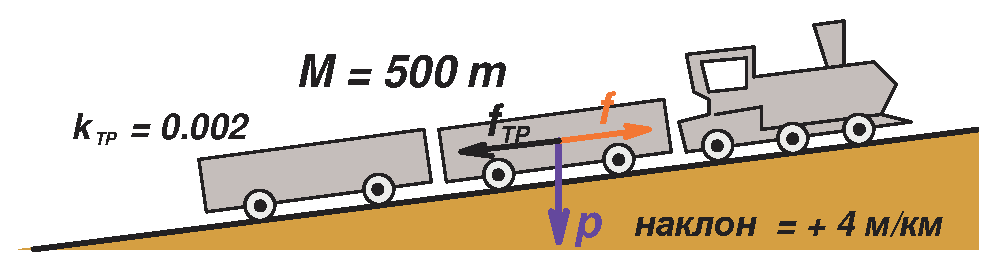
\includegraphics{GP004F04.eps}}
  \end{picture}\\
Решение: скатывающая сила = $p\cdot\sin\alpha\simeq p\cdot\alpha\simeq p\cdot\tan\alpha=0.004p$; она складывается с силой трения $f_{TP}=p\cdot\cos\alpha\cdot k_{TP}\simeq0.002p$.
Поскольку ускорения нет, то все силы скомпенсированы, и $f=0.006p=0.006mg=6\cdot10^{-3}\cdot5\cdot10^5$ кг$\cdot9.8$ м/с$^2=29.4$ кН. Мощность = $f\cdot v=2.94\cdot10^4\cdot72000/3600$ кг$\cdot$м$^2/c^3 = 5.88\cdot10^5$ Вт = 588 кВт $\simeq$ 0.6 МВт $\simeq$ 433 л.с.
\newpage
\underline{\bf Кинетическая энергия}

Работа силы $f$ по разгону тела от $v_1$ до $v_2$ за время $t$: $A=fs$ при ускорении $a=(v_2-v_1)/t$. Сила равна $f=ma=m(v_2-v_1)/t$. Средняя скорость $\bar{v}=(v_1+v_2)/2$, поэтому расстояние $s=t\bar{v}$. Подставив, получим:
   \begin{displaymath}
   A=m\cdot\frac{v_2-v_1}{t}\cdot\frac{v_1+v_2}2\cdot t=\frac{mv_2^2}2-\frac{mv_1^2}2
   \end{displaymath}

\fbox{\parbox{170mm}{\color{blue}Работа силы $f$ численно равна приращению величины $E_k=mv^2/2$, которая называется кинетической энергией.}}\\[2mm]

Если имеется несколько материальных точек, образующих систему, то сказанное справедливо для каждой из них и для всей системы:
   \begin{displaymath}
   E_k=\sum_i\frac{m_iv_i^2}2;\;\;\;\;\;\;\;\;A=\Delta E_k
   \end{displaymath}

\fbox{\parbox{170mm}{\color{blue}Изменение кинетической энергии системы равно работе всех сил, приложенных к материальным точкам, образующим систему.}}\\[2mm]

\underline{\bf Потенциальная энергия}

Силовое поле -- пространство, где на тела действуют силы. Например: однородное гравитационное поле.\\
  \begin{picture}(190,66)(0,0)
   %\put(0,0){\framebox(190,66)[b]{}}
   \put(0,0){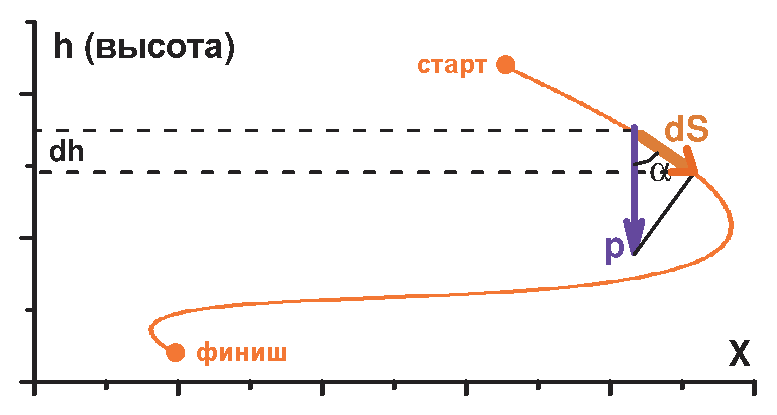
\includegraphics{GP004F05.eps}}
   \put(190,-2){\makebox(0,0)[br]{\parbox{60mm}{С горы съезжает слаломист. Разобьем его трассу на короткие {\bf прямые} кусочки. Работа силы тяжести на каждом i-ом отрезке:
   $dA_i=dS_i\cdot p\cdot\cos\alpha_i$. Но ведь $dS_i\cdot\cos\alpha_i=dh_i$,
   }}}
  \end{picture}\\
поэтому вся (суммарная) работа от старта до финиша составляет
   \begin{displaymath}
   A=\sum_idA_i=\sum_ip\cdot dh_i=p\cdot\sum_idh_i=p\cdot h
   \end{displaymath}
и зависит не от формы или длины пути, а только от перепада высот! Такие силы называются потенциальными.

Введем понятие потенциальной энергии $E_p$ -- такой величины, характери\-зующей положение материальной точки в поле потенциальных сил, что работа при перемещении из одной точки поля в другую будет равна разности значений $E_{p}$ в этих точках:
   \begin{displaymath}
   A_{1,2}=E_{p1}-E_{p2}
   \end{displaymath}
Заметим, что $E_p$ -- не абсолютна, а задает только {\bf разность} по сравнению с какой-то $E_p$, условно принятой за 0.

Для тела с массой $m$ потенциальная энергия в однородном гравитационном поле равна $E_p=mgh$, где $h$ -- уровень относительно некой нулевой высоты.\\

Еще пример: сжимаем пружину с жесткостью $k$.\\
  \begin{picture}(190,110)(0,0)
   %\put(0,0){\framebox(80,110)[b]{}}
   \put(0,0){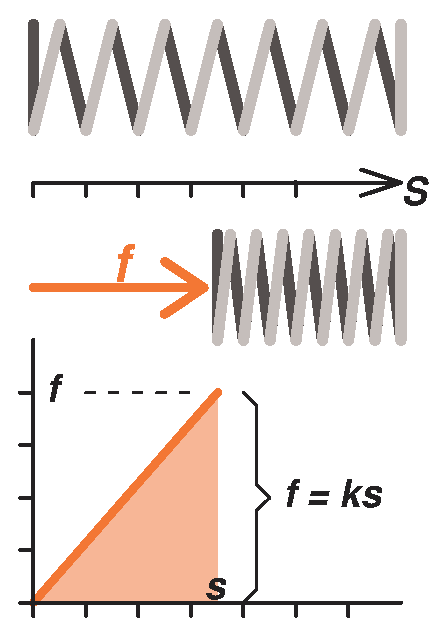
\includegraphics{GP004F06.eps}}
   \put(190,0){\makebox(0,0)[br]{\parbox{110mm}{Сила непостоянна и растет: $f=ks$.  Разбивая отрезок $s$ на короткие кусочки и считая силу на каждом кусочке постоянной, получим, что совершенная работа
   \begin{displaymath}
   A=\sum_i k\cdot s_i\cdot ds_i\;\;\rightarrow\;\;S_\Delta=s\cdot ks/2 = ks^2/2
   \end{displaymath}
или через интеграл:
   \begin{displaymath}
   A=\int_0^sf(s)ds=\int_0^sks\;ds=ks^2/2
   \end{displaymath}
Сжимая пружину, {\bf мы} совершаем работу, а {\bf не пружина}, поэтому мы {\bf увеличиваем} ее потенциальную энергию: $E_p=ks^2/2$.
   }}}
  \end{picture}\\
Как и $E_k$, так же и $E_p$ системы равна сумме $E_{pi}$ частиц, составляющих эту систему. Если система изолирована и если все силы в ней -- потенциальные, то полная работа $A_{1,2}$ при переходе из состояния 1 в состояние 2 зависит только от разности начальной и конечной конфигураций системы, но не от способа перемещений:
   \begin{displaymath}
   A_{1,2}=E_{p1}-E_{p2}
   \end{displaymath}
Это же можно сказать и про разность кинетических энергий системы в состояниях 1 и 2:
   \begin{displaymath}
   A_{1,2}=E_{k2}-E_{k1}
   \end{displaymath}
Сравнивая, получим:
   \begin{displaymath}
   E_{p1}+E_{k1}=E_{p2}+E_{k2}
   \end{displaymath}

\fbox{\parbox{170mm}{\begin{center} \color{red} Закон сохранения механической энергии:\\ \color{blue}
Полная энергия изолированной системы, в которой действуют только потенциальные силы, остается постоянной.
\end{center}
}}\\[2mm]

Пусть $\exists$ замкнутая система с какой-то $E_p=E_0$ и $E_k=0$ (все тела системы покоятся). Тогда при любом движении $E_k$ увеличится ($E_k$ не может быть отрицательной). Это увеличение возможно только за счет уменьшения $E_p$. Если оказалось, что $E_p$ и так минимальна, то: \\

\fbox{\parbox{170mm}{\begin{center}\color{blue}
Замкнутая мех.система, $E_p$ которой имеет минимум и в которой отсутствует движение, находится в состоянии равновесия.
\end{center}
}}\\[2mm]

Что будет, если система неизолированная, и в ней есть трение? Силы в этой системе:
\begin{itemize}
\item внутренние потенциальные
\item внутренние непотенциальные (трение)
\item внешние
\end{itemize}
Тогда работа совершается этими тремя видами сил:
   \begin{displaymath}
   E_{k2}-E_{k1}=A_{1,2}=A_{\rm int}+A_{\rm fr}+A_{\rm ext}
   \end{displaymath}
Из ЗСЭ следует, что {\bf \color{blue} изменение полной механической энергии лю\-бой системы равно сумме работ внешних сил и сил трения}:
   \begin{displaymath}
   E_{2}-E_{1}=A_{\rm fr}+A_{\rm ext}
   \end{displaymath}
\newpage
\underline{\bf Гравитация (силы тяготения).} \\[2mm]
\fbox{\parbox{190mm}{\begin{center} \color{red} Закон всемирного тяготения (Ньютон, 1687 г.):\\ \color{blue}
Всякие тела притягиваются друг к другу с силой,\\ прямо пропорциональной произведению их масс\\ и обратно пропорциональной квадрату расстояния между ними.
\end{center}
}}\\[2mm]
   \begin{displaymath}
   f=G\cdot\frac{m_1 m_2}{r^2}
   \end{displaymath}
Это справедливо только если $r\ll$ размера тел. В противном случе надо интегрировать:\\
  \begin{picture}(190,38)(0,0)
   %\put(0,0){\framebox(190,40)[b]{}}
   \put(0,0){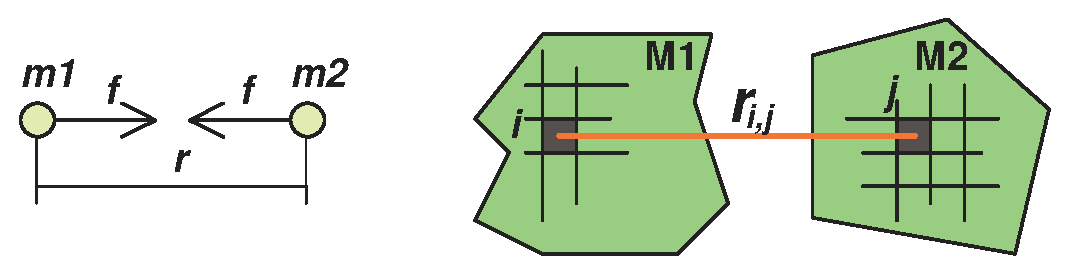
\includegraphics{GP004F07.eps}}
  \end{picture}\\
разбивать каждое тело на мелкие кусочки $\Delta M$, вычислять притяжение между каждой парой кусочков  $\Delta f$ и затем все это суммировать:
   \begin{displaymath}
   f=\sum_{i,j}f_{i,j}=\sum_{i,j}G\cdot\frac{\Delta m_i\cdot\Delta m_j}{r_{i,j}^2}
   \end{displaymath}
Результат интегрирования оказывается таким же только в том случае, когда тела имеют форму однородного шара или сферы -- тогда в качестве $r$ надо просто взять расстояние между {\bf центрами} тел.\\

\underline{\bf Измерение гравитационной постоянной $G$}\\
  \begin{picture}(190,60)(0,0)
   %\put(0,0){\framebox(190,60)[b]{}}
   \put(113,0){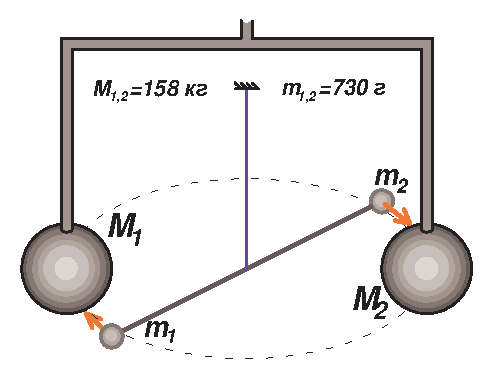
\includegraphics{GP004F08.eps}}
   \put(0,0){\makebox(0,0)[bl]{\parbox{110mm}{Дж.Мичелл (1793): крутильные весы.\\Г.Кавендиш (1798): плотность Земли\\
   С.Пуассон (1811): термин "Гравитационная постоянная"
   \begin{center}
   \fbox{$G=6.67428_{\it 67}\cdot10^{-8}$ дин см$^2$/г$^2$}
   \end{center}
   \begin{center}
   \fbox{$G=6.67428\pm0.00067\cdot10^{-11}$ Н м$^2$/кг$^2$}
   \end{center}
      }}}
  \end{picture}
  \newpage
  У поверхности Земли ускорение тела с массой $m$, вызванное гравитацией:
  \begin{displaymath}
  g=\frac fm=G\cdot\frac{m\cdot M}{m\cdot R^2}=G\cdot\frac M{R^2}
  \end{displaymath}
  Зная $g$ и радиус Земли (из географии, начиная с Архимеда), можно определить массу Земли и ее плотность (что и делал Кавендиш):
  \begin{displaymath}
  M=\frac {g\cdot R^2}G \simeq 5.98\cdot10^{27}\texttt{г};
  \hspace{20mm}\overline{d}=\frac M{\frac43\pi R^3}\simeq5.5\;\texttt{г}/\texttt{см}^3
  \end{displaymath}
  Зная радиус $r$ орбиты Земли относительно Солнца и период ее обращения, можно найти массу Солнца, т.к. гравитация играет роль центростремительной силы:
  \begin{displaymath}
   G\cdot\frac{M\cdot M_\odot}{r^2}=M\cdot r\cdot\frac{4\pi^2}{T^2}\hspace{10mm}
   \Rightarrow\hspace{10mm}
   M_\odot=\frac{4\pi^2}G\cdot\frac{r^3}{T^2}\simeq1.98\cdot10^{33}\;\texttt{г}
  \end{displaymath}
btw: отсюда следует, что для разных планет квадраты периодов обращения относятся как кубы радиусов орбит (третий закон Кеплера).\\

Еще задачка: какой высоты д.б. орбита спутника, чтобы с Земли казалось, что он висит неподвижно?
\\
  \begin{picture}(190,60)(0,0)
   %\put(0,0){\framebox(190,60)[b]{}}
   \put(0,0){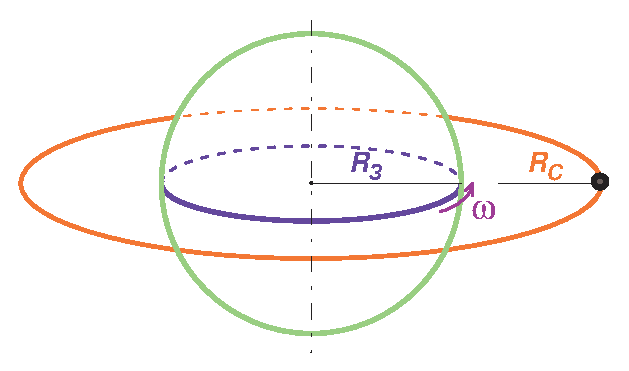
\includegraphics{GP004F09.eps}}
   \put(190,0){\makebox(0,0)[br]{\parbox{80mm}{
  \begin{displaymath}
   G\cdot\frac{M\cdot m}{R_c^2}=m\cdot R_c\cdot\frac{4\pi^2}{T^2}
  \end{displaymath}
  \begin{displaymath}
   R_c^3=\frac{G\cdot M\cdot T^2}{4\pi^2}
  \end{displaymath}
  \begin{displaymath}
   \rule{0mm}{9mm}R_c\simeq\sqrt[3]{75\cdot10^{21}\texttt{м}^3}\simeq
  \end{displaymath}
  \begin{displaymath}
   \simeq4.2\cdot10^7\texttt{м}=42000\;\texttt{км}
  \end{displaymath}
  }}}
  \end{picture}\\[2mm]
Какова потенциальная энергия покоящегося гравитирующего тела на $\infty$?
  \begin{displaymath}
   \left.E_{\infty}=\int\limits_R^\infty f(r)dr=\int\limits_R^\infty \frac{G\cdot M\cdot m}{r^2}dr=
   -\frac{G\cdot M\cdot m}{r}\right|_R^\infty=\frac{G\cdot M\cdot m}{R}
  \end{displaymath}
Если такое тело упадет, то вся $E_p=E_\infty$ перейдет в $E_k=mv^2/2$:
  \begin{displaymath}
   \frac{G\cdot M\cdot m}{R}=\frac{m\cdot v^2}2\hspace{10mm}\Rightarrow\hspace{10mm}
   v=\sqrt{\frac{2GM}{R}}\simeq11.2\;\texttt{км/с}
  \end{displaymath}

\end{document} 